\documentclass[tikz,border=14pt]{standalone}
\usepackage[T1]{fontenc}
\usepackage{lmodern}
\usetikzlibrary{positioning,arrows.meta}
\begin{document}
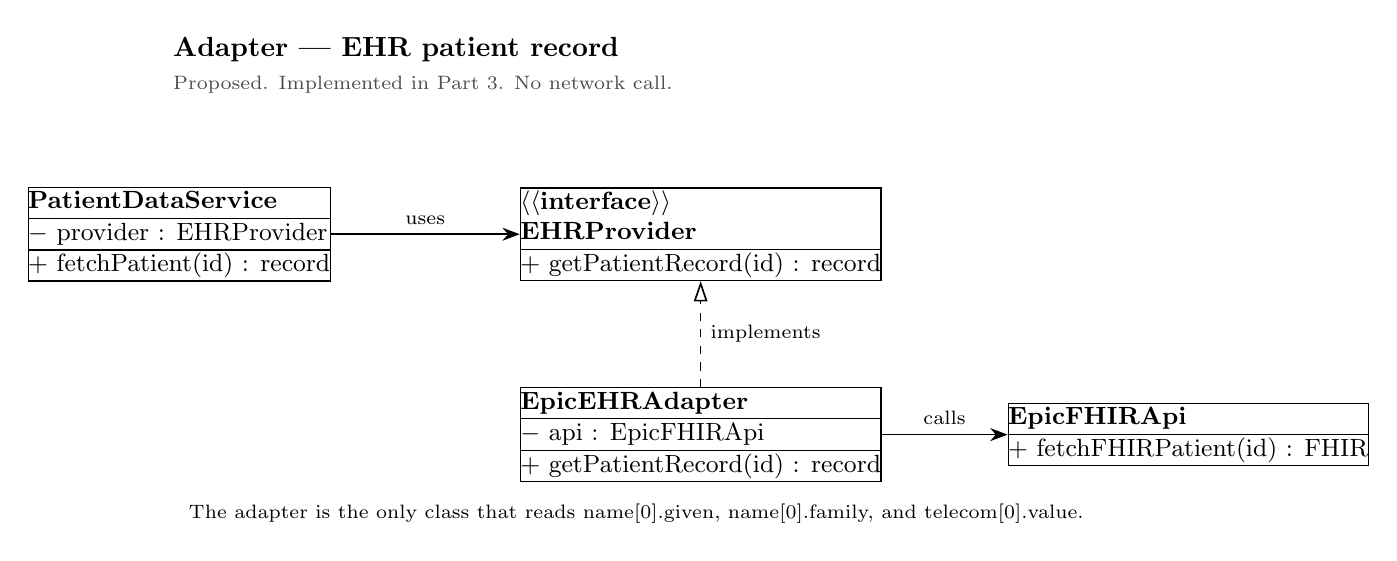
\begin{tikzpicture}[
  font=\small,
  cls/.style={draw, fill=white, inner sep=0pt},
  arr/.style={-{Stealth[length=2.2mm]}, semithick},
  isa/.style={dashed, -{Triangle[open,length=2.6mm]}, semithick}
]
  \node[font=\normalsize\bfseries, anchor=west] at (-0.2,2.35) {Adapter --- EHR patient record};
  \node[font=\scriptsize, anchor=west, text=black!70] at (-0.2,1.9) {Proposed. Implemented in Part 3. No network call.};

  \node[cls] (client) {\begin{tabular}{@{}l@{}}
    \textbf{PatientDataService}\\ \hline
    $-$ provider : EHRProvider\\ \hline
    $+$ fetchPatient(id) : record
  \end{tabular}};
  \node[cls, right=2.4cm of client] (target) {\begin{tabular}{@{}l@{}}
    \textbf{$\langle\langle$interface$\rangle\rangle$}\\
    \textbf{EHRProvider}\\ \hline
    $+$ getPatientRecord(id) : record
  \end{tabular}};
  \node[cls, below=1.35cm of target] (adapter) {\begin{tabular}{@{}l@{}}
    \textbf{EpicEHRAdapter}\\ \hline
    $-$ api : EpicFHIRApi\\ \hline
    $+$ getPatientRecord(id) : record
  \end{tabular}};
  \node[cls, right=1.6cm of adapter] (api) {\begin{tabular}{@{}l@{}}
    \textbf{EpicFHIRApi}\\ \hline
    $+$ fetchFHIRPatient(id) : FHIR
  \end{tabular}};

  \draw[arr] (client.east) -- node[above, font=\scriptsize] {uses} (target.west);
  \draw[isa] (adapter.north) -- node[right, font=\scriptsize] {implements} (target.south);
  \draw[arr] (adapter.east) -- node[above, font=\scriptsize] {calls} (api.west);

  \node[font=\scriptsize, anchor=west, align=left] at (0,-3.55)
    {The adapter is the only class that reads name[0].given, name[0].family, and telecom[0].value.};
\end{tikzpicture}
\end{document}
